\section{Durchführung}
\label{sec:Durchführung}

\begin{figure}[H]
  \centering
  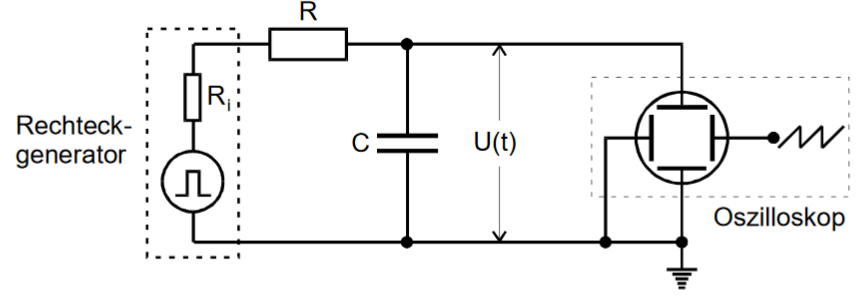
\includegraphics[width=14cm]{Schaltung1.PNG}
  \caption{Schaltung zur Messung der Kondensatorspannung. \cite{sample}}
  \label{fig:Schaltung1}
\end{figure}

Mithilfe eines Funktionsgenerators wird eine Rechteckspannung auf einen RC-Kreis
gegeben. Die Spannung am Kondensator wird, wie in Abbildung \ref{fig:Schaltung1}
zu erkennen, mit einem Oszilloskop abgegriffen und
auf dem Bildschirm ausgegeben. Die Frequenz des Eingangssignals wird so lange variiert,
bis die Auf- und Entladungsvorgänge auf dem Bildschirm deutlich erkennbar sind.
Daraus wird mit der Cursor-Funktion des Oszilloskops die Kondensatorspannung zu verschiedenen Zeitpunkten ermittelt.

Zur Messung der Amplitude der Kondensatorspannung bei periodischer Anregung
wird das Signal auf eine Sinusspannung umgeschaltet. Ihre Amplitude wird mit dem Oszilloskop bestimmt.
Anschließend wird die Frequenz am Funktionsgenerator stückweise erhöht und die entsprechende Amplitude
der Spannung am Kondensator jeweils am Oszilloskop gemessen. Dies wird über drei Zehnerpotenzen der Frequenz
fortgeführt.

\begin{figure}[H]
  \centering
  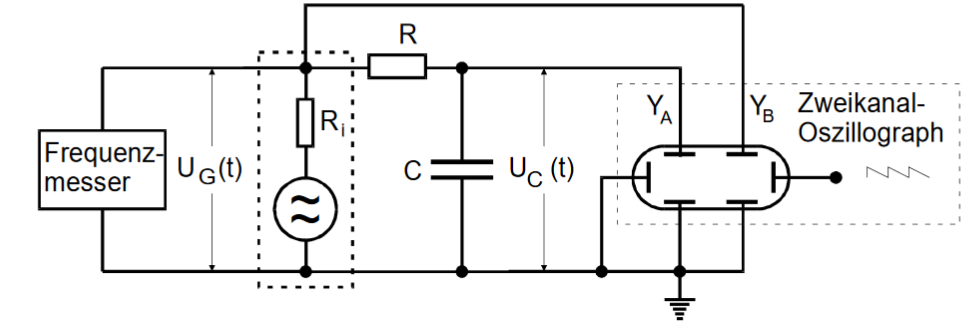
\includegraphics[width=14cm]{Schaltung2.PNG}
  \caption{Schaltung zur Messung der Phasenverschiebung der Spannungen. \cite{sample}}
  \label{fig:Schaltung2}
\end{figure}

Um die Phasenverschiebung der Eingangs- und Kondensatorspannung zu messen,
lässt man beide Spannungen gegen die Zeit auf dem Bildschirm des Oszilloskops ausgeben (siehe Abbildung \ref{fig:Schaltung2}).
Die Frequenz der Eingangsspannung wird wieder stückweise erhöht. Dabei wird
die zeitliche Differenz der Maxima der angezeigten Spannungen (a) sowie die Periodendauer der Eingangsspannung (b)
gemessen (siehe Abbildung \ref{fig:Rechnung}).
Auch hier wird die Frequenz über drei Zehnerpotenzen hinweg erhöht.

\begin{figure}[H]
  \centering
  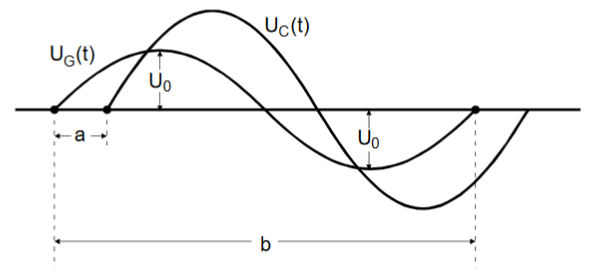
\includegraphics[width=14cm]{Rechnung.PNG}
  \caption{Berechnung der Phasenverschiebung. \cite{sample}}
  \label{fig:Rechnung}
\end{figure}

Anschließend wird die Frequenz auf einen großen Wert gegenüber der Zeitkonstante
des Relaxationsvorgangs eingestellt und erneut werden beide Spannungen auf dem
Bildschirm ausgegeben. Die Eingangsspannung wird nacheinander auf eine Rechteck-, Dreieck-
und Sinusspannung geschaltet und jeweils ein Thermodruck erstellt.
